\documentclass[a4paper, 11pt]{article}

%Comandos para configurar el idioma
\usepackage[spanish,activeacute]{babel}
\usepackage[utf8]{inputenc}
\usepackage[T1]{fontenc} %Necesario para el uso de las comillas latinas.
\usepackage{geometry} % Used to adjust the document margins

%Importante que esta sea la última órden del preámbulo
\usepackage{hyperref}
   \hypersetup{
     pdftitle={Cuestionario de teoría 1},
     pdfauthor={Antonio Álvarez Caballero},
     unicode,
     breaklinks=true,  % so long urls are correctly broken across lines
     colorlinks=true,
     urlcolor=blue,
     linkcolor=darkorange,
     citecolor=darkgreen,
     }

   % Slightly bigger margins than the latex defaults

   \geometry{verbose,tmargin=1in,bmargin=1in,lmargin=1in,rmargin=1in}
\newcommand\fnurl[2]{%
  \href{#2}{#1}\footnote{\url{#2}}%
}


%Paquetes matemáticos
\usepackage{amsmath,amsfonts,amsthm}
\usepackage[all]{xy} %Para diagramas
\usepackage{enumerate} %Personalización de enumeraciones
\usepackage{tikz} %Dibujos
\usepackage{ dsfont }

%Tipografía escalable
\usepackage{lmodern}
%Legibilidad
\usepackage{microtype}

%Código
\usepackage{listings}
\usepackage{color}

\definecolor{dkgreen}{rgb}{0,0.6,0}
\definecolor{gray}{rgb}{0.5,0.5,0.5}
\definecolor{mauve}{rgb}{0.58,0,0.82}

\lstset{frame=tb,
  language=Python,
  aboveskip=3mm,
  belowskip=3mm,
  showstringspaces=false,
  columns=flexible,
  basicstyle={\small\ttfamily},
  numbers=left,
  numberstyle=\tiny\color{gray},
  keywordstyle=\color{blue},
  commentstyle=\color{dkgreen},
  stringstyle=\color{mauve},
  breaklines=true,
  breakatwhitespace=true,
  tabsize=3
}

\title{Cuestionario de teoría 1}
\author{Antonio Álvarez Caballero\\
    \href{mailto:analca3@correo.ugr.es}{analca3@correo.ugr.es}}
\date{\today}

\theoremstyle{definition}
\newtheorem{ejercicio}{Ejercicio}
\newtheorem{cuestion}{Cuestión}
\newtheorem*{solucion}{Solución}
\newtheorem*{bonus}{BONUS}



%%%%%%%% New sqrt
\usepackage{letltxmacro}
\makeatletter
\let\oldr@@t\r@@t
\def\r@@t#1#2{%
\setbox0=\hbox{$\oldr@@t#1{#2\,}$}\dimen0=\ht0
\advance\dimen0-0.2\ht0
\setbox2=\hbox{\vrule height\ht0 depth -\dimen0}%
{\box0\lower0.4pt\box2}}
\LetLtxMacro{\oldsqrt}{\sqrt}
\renewcommand*{\sqrt}[2][\ ]{\oldsqrt[#1]{#2} }
\makeatother

%%%%%%%%%%%%%%%%%%%%%%%%%%%%%%%%%%%%%%%%%%%%%

%%%%%%%%%%%% Norm
\newcommand{\norm}[1]{\left\lVert#1\right\rVert}
%%%%%%%%%%%%%%%%%

%%%%%%%%%%% Ceil
\usepackage{mathtools}
\DeclarePairedDelimiter{\ceil}{\lceil}{\rceil}
%%%%%%%%%%%%%%%%%%%%%%%%%%%%%%%%%%%%%%%%%%%

\begin{document}

  \maketitle

  \section{Cuestiones}

  \begin{cuestion}
    Identificar, para cada una de las siguiente tareas, qué tipo de aprendizaje automático es el adecuado (supervisado, no supervisado, por refuerzo) y los datos de aprendizaje que deberíamos usar. Si una tarea se ajusta a más de un tipo, explicar cómo y describir los datos para cada tipo.
    \begin{enumerate}
      \item[a)] Categorizar un grupo de animales vertebrados en pájaros, mamíferos, reptiles, aves y anfibios.
      \item[b)] Clasificación automática de cartas por distrito postal.
      \item[c)] Decidir si un determinado índice del mercado de valores subirá o bajará dentro de un periodo de tiempo fijado.
    \end{enumerate}

  \end{cuestion}

  \begin{solucion}
    Los tipos de aprendizaje son:
    \begin{enumerate}
      \item[a)] Aprendizaje supervisado. Lo importante aquí es el conjunto de datos, ya que cada uno de estas clases tiene características bastante bien definidas (pelo, plumas, número de patas, número de alas, piel seca o húmeda, escamas, órganos respiratorios, \ldots). Como existe alguna pequeña superposición entre clases (un ornitorrinco es un mamífero que pone huevos, por ejemplo) sería difícil una aproximación por diseño.
      \item[b)] Aprendizaje no supervisado. Aquí no hace falta que se sepa realmente la etiqueta de los datos, simplemente con que el sistema sea capaz de agrupar las cartas que pertenezcan al mismo distrito postal (que tengan el mismo número manuscrito).
      \item[c)] Por refuerzo. No siempre podemos basarnos en datos que ya tenemos para decidir esto (los datos de hace 4 años no tienen por qué ser relevantes ahora), por lo que una aproximación por refuerzo irá aprendiendo sobre la marcha con la actividad actual del mercado de valores.
    \end{enumerate}
  \end{solucion}

  \begin{cuestion}
    ¿Cuáles de los siguientes problemas son más adecuados para una aproximación por aprendizaje y cuáles más adecuados para una aproximación por diseño? Justificar la decisión.
    \begin{enumerate}
      \item[a)] Determinar el ciclo óptimo para las luces de los semáforos en un cruce con mucho tráfico.
      \item[b)] Determinar los ingresos medios de una persona a partir de sus datos de nivel de educación, edad, experiencia y estatus social.
      \item[c)] Determinar si se debe aplicar una campaña de vacunación contra una enfermedad.
    \end{enumerate}

  \end{cuestion}

  \begin{solucion}
    Las aproximaciones son:
    \begin{enumerate}
      \item[a)] Aproximación por diseño. Este es un problema que puede llegar a ser crítico si se produce algún fallo, luego una aproximación por diseño (exhaustivo) dará mejor resultado en una primera instancia que una aproximación por aprendizaje.
      \item[b)] Aproximación por aprendizaje. Los ingresos medios de una persona no están directamente relacionados con los datos proporcionados, luego deberíamos intentar aprender de esos datos y realizar algún modelo que nos permita \emph{predecir} este dato de forma aceptable.
      \item[c)] Aproximación por aprendizaje. Se podría realizar aprendizaje sobre algún conjunto de datos que incluyera (por ejemplo) un factor de contagio de la enfermedad, probabilidad de secuelas críticas, etc... para, dada una enfermedad, poder decidir si es necesaria o no dicha campaña.
    \end{enumerate}
  \end{solucion}

  \begin{cuestion}
  Construir un problema de \emph{aprendizaje desde datos} para un problema de selección de fruta en una explotación agraria (ver transparencias de clase). Identificar y describir cada uno de sus elementos formales. Justificar las decisiones.
  \end{cuestion}

  \begin{solucion}
    Determinemos los aspectos clave:
    \begin{itemize}
      \item $\mathcal{X}$: Un espacio n-dimensional con las características de los mangos. Podríamos tomar un espacio 5-dimensional donde las características son (color, tamaño, textura, tiempo de maduración, peso).
      \item $\mathcal{Y}$: Podemos usar clasificación binaria: 1 si el mango es bueno y -1 si no lo es.
      \item Conjunto de entrenamiento: Un análisis previo de la cosecha midiendo cada una de las características propuestas y determinando si el mango es bueno o no.
      \item $\mathcal{H}$: En principio podríamos intentar buscar en las funciones lineales, ya que son las más sencillas. Si no consiguiéramos un buen clasificador, ya iríamos subiendo la complejidad de estas funciones en busca de un clasificador aceptable.
    \end{itemize}
  \end{solucion}

  \begin{cuestion}
  Suponga un modelo PLA y un dato $x(t)$ mal clasificado respecto de dicho modelo. Probar que la regla de adaptación de pesos del PLA es un movimiento en la dirección correcta para clasificar bien $x(t)$.

  \end{cuestion}

  \begin{solucion}
    Definimos primero el término $y(t)w^T(t)x(t)$ como, informalmente,  el resultado de clasificar $x(t)$ con $w(t)$. Claramente es $>0$ si está bien clasificado y $<0$ si no lo está, ya que si está bien clasificado tenemos que $y(t) = sign(w^T(t)x(t))$, por lo cual su producto es positivo, y en caso contrario $y(t) \neq sign(w^T(t)x(t))$, lo cual su producto es negativo.

    Usando esto, veamos que $y(t)w^T(t+1)x(t) > y(t)w^T(t)x(t)$. Es claro ya que      si expandimos el primer miembro con la regla de actualización del \emph{PLA} vemos que:

    \[
    y(t)w^T(t+1)x(t) = y(t){\big( w(t)+y(t)x(t) \big)}^T x(t) = y(t)w^T(t)x(t) + \underbrace{{\norm{x(t)}}^2}_{>0}
    \]

    Por lo cual la desigualdad de arriba queda clara. Con esto deducimos que la clasificación de $x(t+1)$ siempre será \emph{mejor} que la de $x(t)$, ya que el valor de su clasificación es mayor, lo cual hace que pueda superar a $0$, implicando que el dato estaría bien clasificado. Podría no superar a $0$, pero en tal caso estaría más cerca de estar bien clasificado.
  \end{solucion}

  \begin{cuestion}
  Considere el enunciado del ejercicio 2 de la sección FACTIBILIDAD DEL APRENDIZAJE de la relación de apoyo.
  \begin{enumerate}
  \item[a)] Si $p=0,9$, ¿cuál es la probabilidad de que $S$ produzca una hipótesis mejor que $C$?
  \item[b)] ¿Existe un valor de $p$ para el cual es más probable que $C$ produzca una hipótesis mejor que $S$?
  \end{enumerate}
  \end{cuestion}

  \begin{solucion}
    Las soluciones son:
    \begin{enumerate}
      \item[a)] Queremos determinar cuál es la probabilidad de que el error fuera de la muestra sea menor para $S$ que para $C$:
        \begin{equation*}
          \begin{split}
            P\left[E_{out}(S(\mathcal{D})) < E_{out}(C(\mathcal{D}))  \right] &=           P\left[E_{out}(h_1) < E_{out}(h_2)  \right] \\
            &= P\left[P\left[f(x) \neq h_1\right] < P\left[f(x) \neq h_2\right]  \right] \\
            &= P\left[P\left[f(x) = -1\right] < P\left[f(x) =+1\right]  \right] \\
            &= P\left[1-p < p \right] = P\left[0.1 < 0.9 \right] = 1
          \end{split}
        \end{equation*}
      \item[b)] En este caso  razonamos igual que en el anterior, pero dándole la vuelta a la desigualdad y sin determinar $p$:
      \begin{equation*}
        \begin{split}
          P\left[E_{out}(S(\mathcal{D})) > E_{out}(C(\mathcal{D}))  \right] &=           P\left[E_{out}(h_1) > E_{out}(h_2)  \right] \\
          &= P\left[P\left[f(x) \neq h_1\right] > P\left[f(x) \neq h_2\right]  \right] \\
          &= P\left[P\left[f(x) = -1\right] > P\left[f(x) =+1\right]  \right] \\
          &= P\left[1-p > p \right] = P\left[ 0.5 > p \right] = 1
        \end{split}
      \end{equation*}
      Es claro que dicha probabilidad es $1$ si y solamente si $p < 0.5$
    \end{enumerate}
  \end{solucion}

  \begin{cuestion}
  La desigualdad de Hoeffding modificada nos da una forma de caracterizar el error de generalización con una cota probabilística
  \[
  \mathds{P}[|E_{out}(g) - E_{in}(g)| > \epsilon] \leq 2Me^{-2N \epsilon^2}
  \]
  para cualquier $\epsilon > 0$. Si fijamos $\epsilon=0,05$ y queremos que la cota probabilística $2Me^{-2N^2 \epsilon}$ sea como máximo $0,03$, ¿cuál será el valor más pequeño de $N$ que verifique estas condiciones si $M=1$? Repetir para $M=10$ y para $M=100$.

  \end{cuestion}

  \begin{solucion}
    Sólo tenemos que despejar $N$ de la ecuación para conseguir los valores deseados. Como queremos que la cota sea $0.03$, igualamos y despejamos:

      \[
      2Me^{-2N\epsilon^2} = 0.03
      \]

      \[
      e^{-2N\epsilon^2} = \frac{0.015}{M}
      \]

      \[
      -2N\epsilon^2 = log\left(\frac{0.015}{M}\right)
      \]

      \[
      N = \ceil{-log\left(\frac{0.015}{M}\right) \frac{1}{2\epsilon^2}}
      \]

      Ahora sólo tenemos que introducir $\epsilon = 0.05$ y los distintos valores de $M$.

      $$M =  1 \rightarrow N =  840$$
      $$M =  10 \rightarrow N =  1301$$
      $$M =  100 \rightarrow N =  1761$$
      $$M =  1000 \rightarrow N =  2222$$

  \end{solucion}

  \begin{cuestion}
  Consideremos el modelo de aprendizaje \emph{M-intervalos} donde $h: \mathbb{R} \rightarrow \{-1, +1\}$ y $h(x)=+1$ si el punto está dentro de cualquiera de $m$ intervalos arbitrariamente elegidos y $h(x)=-1$ en otro caso. ¿Cuál es el más pequeño punto de ruptura para este conjunto de hipótesis?

  \end{cuestion}

  \begin{solucion}
    El modelo de \emph{M-intervalos} es una generalización del modelo del \emph{intervalo}. Sabemos que para este modelo el punto de ruptura es $k = 3$. Veamos entonces si conseguimos alguna función lineal $aM + b; a,b \in \mathbb{N}$ que nos dé dicho valor de $k$ para el caso $M = 1$. Claramente los posibles valores son $a = 2 \bigwedge b = 1$ o $a = 1 \bigwedge b = 2$. Probamos con el primero, dándonos la función $2M+1$, viendo si el modelo es capaz de clasificar completamente $2M$ dicotomías y no puede con $2M+1$.

    Claramente el modelo puede separar correctamente un conjunto de $2M$ puntos. Supongamos que tenemos $M$ 1's y $M$ -1's. Recubriendo cada uno con un intervalo (sin alcanzar ningún $-1$) podemos clasificar cualquier dicotomía de este conjunto. Al haber separado un conjunto, podemos decir que NO es punto de ruptura.

    Veamos para un conjunto con $2M+1$ puntos: la condición que necesitamos es que NO pueda clasificar todas las dicotomías de ningún conjunto. Es claro que no se puede: tomamos una dicotomía con $M$ -1's y $M+1$ 1's. Si estos puntos están alternados $(1,-1,1,\ldots,1,-1,1)$, no podemos clasficarlos con $M$ intervalos.
  \end{solucion}

  \begin{cuestion}
  Suponga un conjunto de $k^*$ puntos $x_1,x_2,...,x_{k^*}$ sobre los cuales la clase $H$ implementa $<2^{k^*}$ dicotomías. ¿Cuáles de las siguientes afirmaciones son correctas?
  \begin{enumerate}
  \item[a)] $k^*$ es un punto de ruptura
  \item[b)] $k^*$ no es un punto de ruptura
  \item[c)] todos los puntos de ruptura son estrictamente mayores que $k^*$
  \item[d)] todos los puntos de ruptura son menores o iguales a $k^*$
  \item[e)] no conocemos nada acerca del punto de ruptura
  \end{enumerate}

  \end{cuestion}

  \begin{solucion}
    La respuesta correcta es la e). Para llegar a una conclusión tendría que ser \emph{para todo conjunto de} $k^*$ \emph{puntos}.
  \end{solucion}

  \begin{cuestion}
  Para todo conjunto de $k^*$ puntos, $H$ implementa $<2^{k^*}$ dicotomías. ¿Cuáles de las siguientes afirmaciones son correctas?
  \begin{enumerate}
  \item[a)] $k^*$ es un punto de ruptura
  \item[b)] $k^*$ no es un punto de ruptura
  \item[c)] todos los $k \geq k^*$ son puntos de ruptura
  \item[d)] todos los $k < k^*$ son puntos de ruptura
  \item[e)] no conocemos nada acerca del punto de ruptura
  \end{enumerate}
  \end{cuestion}

  \begin{solucion}
    Las respuestas correctas con a) y c). Como son todos los conjuntos, $2^{k^*}$ acota las dicotomías que implementa $H$. Además, cualquier valor mayor a dicho $k^*$ también lo acotará.
  \end{solucion}

  \begin{cuestion}
  Si queremos mostrar que $k^*$ es un punto de ruptura, ¿cuáles de las siguientes afirmaciones nos servirían para ello?:
  \begin{enumerate}
  \item[a)] Mostrar que existe un conjunto de $k^*$ puntos $x_1,\ldots,x_{k^*}$ que $H$ puede separar (\emph{shatter}).
  \item[b)] Mostrar que $H$ puede separar cualquier conjunto de $k^*$ puntos.
  \item[c)] Mostrar un conjunto de $k^*$ puntos $x_1,\ldots,x_{k^*}$ que $H$ no puede separar.
  \item[d)] Mostrar que $H$ no puede separar ningún conjunto de $k^*$ puntos.
  \item[e)] Mostrar que $m_H(k)=2^{k^*}$
  \end{enumerate}
  \end{cuestion}

  \begin{solucion}
    La solución es d). Si separara alguno, estaríamos en el caso de la cuestión 8. Si los separara todos, en el caso de la 9.
  \end{solucion}

  \begin{cuestion}
  Para un conjunto $H$ con $d_{VC}=10$, ¿qué tamaño muestral se necesita (según la cota de generalización) para tener un $95\%$ de confianza de que el error de generalización sea como mucho $0,05$?

  \end{cuestion}

  \begin{solucion}
    Tal y como se explica en las transparencias, se resolverá la cota del tamaño de la muestra iterativamente sobre la fórmula apropiada.

    \lstinputlisting{complejidad.py}

    El tamaño resultado de ejecutar este script es de 452957.
  \end{solucion}

  \begin{cuestion}
  Consideremos un escenario de aprendizaje simple. Supongamos que la dimensión de entrada es uno. Supongamos que la variable de entrada $x$ está uniformemente distribuida en el intervalo $[-1,1]$ y el conjunto de datos consiste en 2 puntos $\{x_1,x_2\}$ y que la función objetivo es $f(x)=x^2$. Por tanto el conjunto de datos completo es $\mathcal{D}=\{(x_1,x_1^2), (x_2,x_2^2)\}$. El algoritmo de aprendizaje devuelve la línea que ajusta estos dos puntos como $g$ (i.e. $H$ consiste en funciones de la forma $h(x)=ax+b$).
  \begin{enumerate}
  \item[a)] Dar una expresión analítica para la función promedio $\overline{g}(x)$.
  \item[b)] Calcular analíticamente los valores de $E_{out}$, \emph{bias} y \emph{var}.
  \end{enumerate}
  \end{cuestion}

  \begin{solucion}
    Primero definamos explícitamente $g^{(\mathcal{D})}(x)$. Como es la recta que corta a los puntos de $\mathcal{D}$, se define en forma punto pendiente como $g^{(\mathcal{D})}(x) = \frac{x_2^2-x_1^2}{x_2-x_1}(x-x_1) + x_1^2$. Simplificando el primer término con la identidad suma por diferencia nos queda $g^{(\mathcal{D})}(x) = (x_2+x_1)(x-x_1) + x_1^2$.

    Sabemos por definición que $\overline{g}(x) = \mathbb{E}_\mathcal{D}\left[ g^{(\mathcal{D})}(x) \right]$. Como la distribución de los puntos es uniforme, su función de densidad es $f(x) = \frac{1}{\lambda(\mathcal{D})}$, con $\lambda$ la medida del conjunto (que en este caso obviamente es 4). Además, $x_1$ y $x_2$ son independientes. Por tanto la esperanza quedaría:


    \begin{equation*}
      \begin{split}
        \overline{g}(x) = \mathbb{E}_\mathcal{D}\left[ g^{(\mathcal{D})}(x) \right] = \mathbb{E}_\mathcal{D}\left[ (x_2+x_1)(x-x_1) + x_1^2 \right] &=            \mathbb{E}_\mathcal{D}\left[ x(x_1+x_2) - x_1x_2 \right] \\
        &= x\mathbb{E}_\mathcal{D}\left[ x_1+x_2 \right] - \mathbb{E}_\mathcal{D}\left[ x_1x_2 \right] \\
        &= x\big( \mathbb{E}_\mathcal{D}\left[ x_1 \right] + \mathbb{E}_\mathcal{D}\left[ x_2 \right] \big) - \mathbb{E}_\mathcal{D}\left[ x_1 \right] \mathbb{E}_\mathcal{D}\left[ x_2 \right]
      \end{split}
    \end{equation*}

    Como el espacio de medida es simétrico (es un cuadrado), es claro que

    $$\mathbb{E}_\mathcal{D}\left[ x_1 \right] = \mathbb{E}_\mathcal{D}\left[ x_2 \right]$$

    Por tanto, veamos cuánto vale $\mathbb{E}_\mathcal{D}\left[ x_1 \right]$. Es claro que vale 0 ya que

    $$ \mathbb{E}_\mathcal{D}\left[ x_1 \right] = \frac{1}{4}\int_{-1}^1 \int_{-1}^1 \! x_1 \, \mathrm{d}x_1 \mathrm{d}x_2 = \frac{1}{4} \int_{-1}^1 \frac{x_1^2}{2} \biggr\rvert_{-1}^1 \mathrm{d}x_2 = 0 $$

    Por tanto, sustituyendo todas las esperanzas en la fórmula de arriba, nos queda:

    $$\overline{g}(x) = 0 $$

    Ahora calculemos $E_{out}$, \emph{bias} y \emph{var}. Aplicamos sus respectivas definiciones:

    $$ bias(x) = {(\overline{g}(x) - f(x))}^2 = f(x)^2 = x^4 $$
    $$ var(x) = \mathbb{E}_\mathcal{D}\left[ {(g^{(\mathcal{D})}(x) - \overline{g}(x) )}^2 \right] = \mathbb{E}_\mathcal{D}\left[ {g^{(\mathcal{D})}(x)}^2 \right] $$

    Esta varianza se calcula utilizando el módulo de Python \emph{Sympy}, que es un completo paquete de cálculo simbólico.

    \begin{lstlisting}
      import sympy

      sympy.init_session()
      x1, x2 = symbols('x1 x2')

      print(integrate( ((x1+x2)*x - x1*x2) ** 2, (x1,-1,1),(x2,-1,1) ) )
    \end{lstlisting}
    Nos devuelve

    $$ \frac{8 x^{2}}{3} + \frac{4}{9}$$

    Como queremos la esperanza en el conjunto y no solamente la integral, debemos multiplicarlo por la función densidad (la inversa de la medida del conjunto).

    $$var(x) = \mathbb{E}_\mathcal{D}\left[ {(g^{(\mathcal{D})}(x) - \overline{g}(x) )}^2 \right] = \mathbb{E}_\mathcal{D}\left[ {g^{(\mathcal{D})}(x)}^2 \right] = \frac{1}{4} \left(\frac{8 x^{2}}{3} + \frac{4}{9} \right) = \frac{2 x^{2}}{3} + \frac{1}{9}$$

    Ahora sólo nos queda $E_{out}$. La esperanza en x se calcula igual que en $\mathcal{D}$, pero en este caso la medida del conjunto $[-1,1]$ es $2$.

    $$ E_{out} = \mathbb{E}_\mathcal{D}\left[E_{out}(g^{(\mathcal{D})}) \right] = \mathbb{E}_x \left[ bias(x) + var(x)  \right] = \underbrace{\mathbb{E}_x \left[ bias(x) \right]}_{= \frac{1}{5}} + \underbrace{\mathbb{E}_x \left[ var(x)  \right]}_{=\frac{1}{3}} =  \frac{8}{15}$$

  \end{solucion}

  %%%% BONUS %%%%

  \begin{bonus}
    Considere el enunciado del ejercicio 2 de la sección ERROR Y RUIDO de la relación de apoyo.
    \begin{itemize}
      \item[a)] Si su algoritmo busca la hipótesis $h$ que minimiza la suma de los valores absolutos de los errores de la muestra,

      \[
      E_{in}(h) = \sum_{n=1}^N{|h-y_n|}
      \]
      entonces mostrar que la estimación será la mediana de la muestra, $h_{med}$ (cualquier valor que deje la mitad de la muestra a su derecha y la mitad a su izquierda)

      \item[b)] Suponga que $y_n$ es modificado como $y_n + \epsilon$, donde $\epsilon \rightarrow \infty$. Obviamente el valor de $y_n$ se convierte en un punto muy alejado de su valor original. ¿Cómo afecta esto a los estimadores dados por $h_{mean}$ y $h_{med}$?
    \end{itemize}
  \end{bonus}

  \begin{solucion}

    Resolvemos por partes:
    \begin{enumerate}

      \item[a)]Primero colocamos $h$ al inicio del conjunto de datos, $h \leq y_1 \leq \ldots \leq y_n$. Descomponemos la sumatoria (los datos están ordenados) y nos queda:

      $$ E_{in}(h) = \sum_{n=1}^N{|h-y_n|} = \sum_{n=1}^N{(y_n-h)} = \sum_{n=1}^N{y_n} - \sum_{n=1}^N{h} = \sum_{n=1}^N{y_n} - Nh$$

      Derivamos e igualamos a cero para encontrar un extremo:

      $$E_{in}'(h) = -N = 0 $$

      Lo cual es una contradicción, ya que sería el caso de no haber datos. El caso colocando $h$ al final del conjunto de datos es recíproco, saldría $N=0$.

      Ahora colocamos $h$ en $y_1 \leq \ldots \leq y_k \leq h \leq y_{k+1} \leq \ldots \leq y_N$. Descomponemos la sumatoria gracias a que todos los valores están ordenados:

      $$E_{in}(h) = \sum_{n=1}^N{|h-y_n|} = \sum_{n=1}^k{(h-y_n)} + \sum_{n=k+1}^N{(y_n-h)} = \sum_{n=1}^k{h}-\sum_{n=1}^k{y_n} + \sum_{n=k+1}^N{y_n}-\sum_{n=k+1}^N{h}$$

      $$E_{in}(h)= kh-\sum_{n=1}^k{y_n} + \sum_{n=k+1}^N{y_n}-(N-k)h$$

      Derivamos e igualamos a cero.

      $$E_{in}'(h) = k - (N - k) = 2k - N = 0 \Leftrightarrow k = \frac{N}{2}$$

      Hemos determinado que para que $h$ PUEDA ser un mínimo, debe estar entre $y_k$ y $y_{k+1}$ con $k=\frac{N}{2}$, que hace que esté en medio de todos los datos (deja $k$ datos a la izquierda y $k$ a la derecha). Es claro que es un mínimo ya que si $k < \frac{N}{2}$, $E_{in}'(h) < 0$ y si $k > \frac{N}{2}$, $E_{in}'(h) > 0$, luego la función decrece y luego crece.    Por tanto, este valor es la mediana.

      En el caso de que $N$ sea impar, realizamos el mismo método de arriba, pero como paso preliminar hacemos lo siguiente: el dato colocado en la posición $\frac{N+1}{2}$ lo duplicamos en la lista de datos. Así, el mínimo de la función no cambiaría de posición (sólo trasladamos la función hacia arriba). Al realizar el procedimiento de arriba, tendríamos que para que $h$ sea mínimo debe estar entre el dato $\frac{N+1}{2}$ y $\frac{N+1}{2} + 1$. Pero al haber duplicado el dato $\frac{N+1}{2}$, tenemos que

      $$ y_{\frac{N+1}{2}} = h = y_{\frac{N+1}{2}+1} $$

      Luego $h$ debe estar en la posición de la mediana.

      \item[b)] Para el valor de la mediana, es claro que se queda igual, ya que la mediana es un valor posicional, no depende de los valores de los datos.

      Para el caso de la media procedemos como sigue: esta sería la expresión de la media para el conjunto de datos original y modificado:

      $$ h_{med} = \frac{1}{N} \sum_{n=1}^N{y_n} = \frac{1}{N} \left( \sum_{n=1}^{N-1}{y_n} + y_N \right)$$

      $$ h_{med}' = \frac{1}{N} \sum_{n=1}^N{y_n'} = \frac{1}{N} \left( \sum_{n=1}^{N-1}{y_n} + y_N + \epsilon \right)$$

      Si restamos ambas expresiones nos queda:

      $$ h_{med}' - h_{med} = \frac{1}{N} \left(\epsilon \right)$$

      Luego si $\epsilon \rightarrow \infty$, esta diferencia diverge.

    \end{enumerate}

  \end{solucion}

  \begin{bonus}
    Considere el ejercicio 12.
    \begin{itemize}
      \item[a)] Describir un experimento que podamos ejecutar para determinar (numéricamente) $\overline{g}(x)$, $E_{out}$, \emph{bias} y \emph{var}.

      \item[b)] Ejecutar el experimento y dar los resultados. Comparar $E_{out}$ con \emph{bias+var}. Dibujar en unos mismos ejes $g(x)$, $E_{out}$ y $f(x)$.
    \end{itemize}
  \end{bonus}

  \begin{solucion}
    Apliquemos las fórmulas que tenemos en las transparencias. Como es una media aritmética, lo aplicaremos sobre varios conjuntos de datos, cada vez más grandes, para ver su comportamiento. Usaremos Python y sus librería \emph{NumPy} y \emph{SymPy} para cálculo numérico y simbólico.

    Se hicieron algunas pruebas con 10000 y 100000 datos, pero se desecharon pronto porque era demasiado tiempo de cómputo (hasta 3 minutos sólo para calcular la $\overline{g}(x)$), y con 1000 datos también se ha probado (la salida está en el propio código), pero se ha dejado un tamaño de 100 datos para que el cálculo sea rápido, aunque el $E_{out}$ mejora un 5\% en el caso de 1000 datos.

    Seguramente la solución propuesta no es la más eficiente, pero ha sido rápido de escribir. La idea es tomar 100 muestras aleatorias en $[-1,1]$ e ir calculando esperanzas como medias de funciones o de valores, según el caso. Primero calculamos $\overline{g}(x)$, luego se calcula $bias(x)$ y su esperanza, $varianza(x)$ y su esperanza y por último $E_{out}^{\mathcal(D)}$ y su esperanza, y se compara con $bias+varianza$.

    \lstinputlisting{bias-var.py}

    Aquí la salida con 100 datos.

    \begin{verbatim}
      g_media(x) = -0.0240978062019481*x - 0.0506736366465499
      Bias = 0.237413164642445
      Calculando varianza...
      Varianza = 0.365272167591865
      Calculando Eout_D...
      Eout_D calculado, ahora la esperanza...
      Eout con esperanza = 0.602685332234309  Eout usando bias + var = 0.602685332234310
      Tiempo transcurrido = 5.334069013595581 segundos
    \end{verbatim}


    Y aquí con 1000 datos.

    \begin{verbatim}
      g_media(x) = -0.0116637213459665*x - 0.0155484354190228
      Bias = 0.211474902374281
      Calculando varianza...
      Varianza = 0.332779003271147
      Calculando Eout_D...
      Eout_D calculado, ahora la esperanza...
      Eout con esperanza = 0.544253905645427  Eout usando bias + var = 0.544253905645428
      Tiempo transcurrido = 98.63339281082153 segundos

    \end{verbatim}

    Aquí la gráfica para el caso de 100 datos.

    \centerline{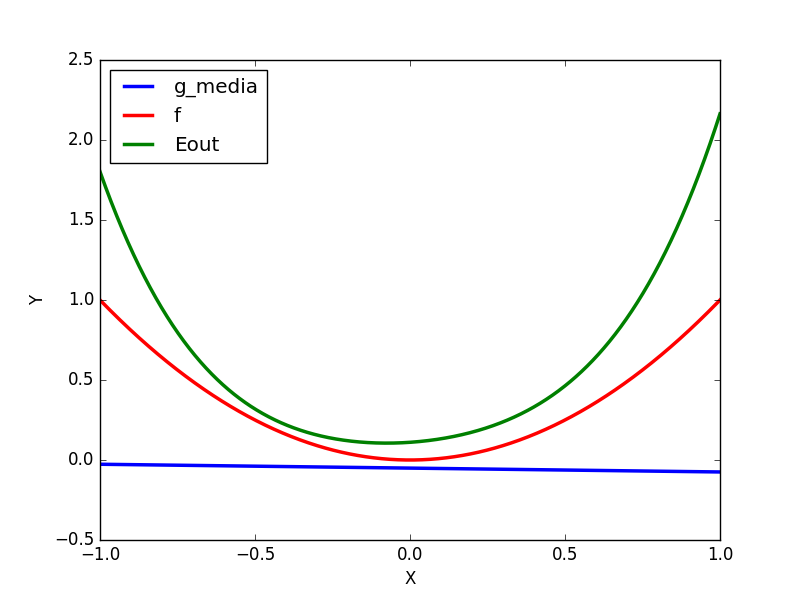
\includegraphics[width=0.7\textwidth]{salida_bonus.png}}

    Los resultados nos aclaran varias cosas: la importante equivalencia entre $E_{out}$ y $bias+varianza$ y la poca diferencia entre la solución analítica ($bias=\frac{1}{5}$ y $var=\frac{1}{3}$) y la numérica usando sólo 100 datos. Con 1000 datos la diferencia es poco apreciable, aunque el tiempo de cómputo ha sido bastante mayor (las operaciones simbólocas son bastante costosas).

    Con la gráfica podemos ver lo que intuitivamente está claro: el error que se comete al aproximar una parábola con una recta es cada vez mayor cuanto más nos separamos del vértice de la parábola.



  \end{solucion}

\end{document}
